\chapter{Experiments}\label{chap:experiments}

% \begin{figure}[t]
    \begin{centering}
        \subfloat[Some cool graphic]
        {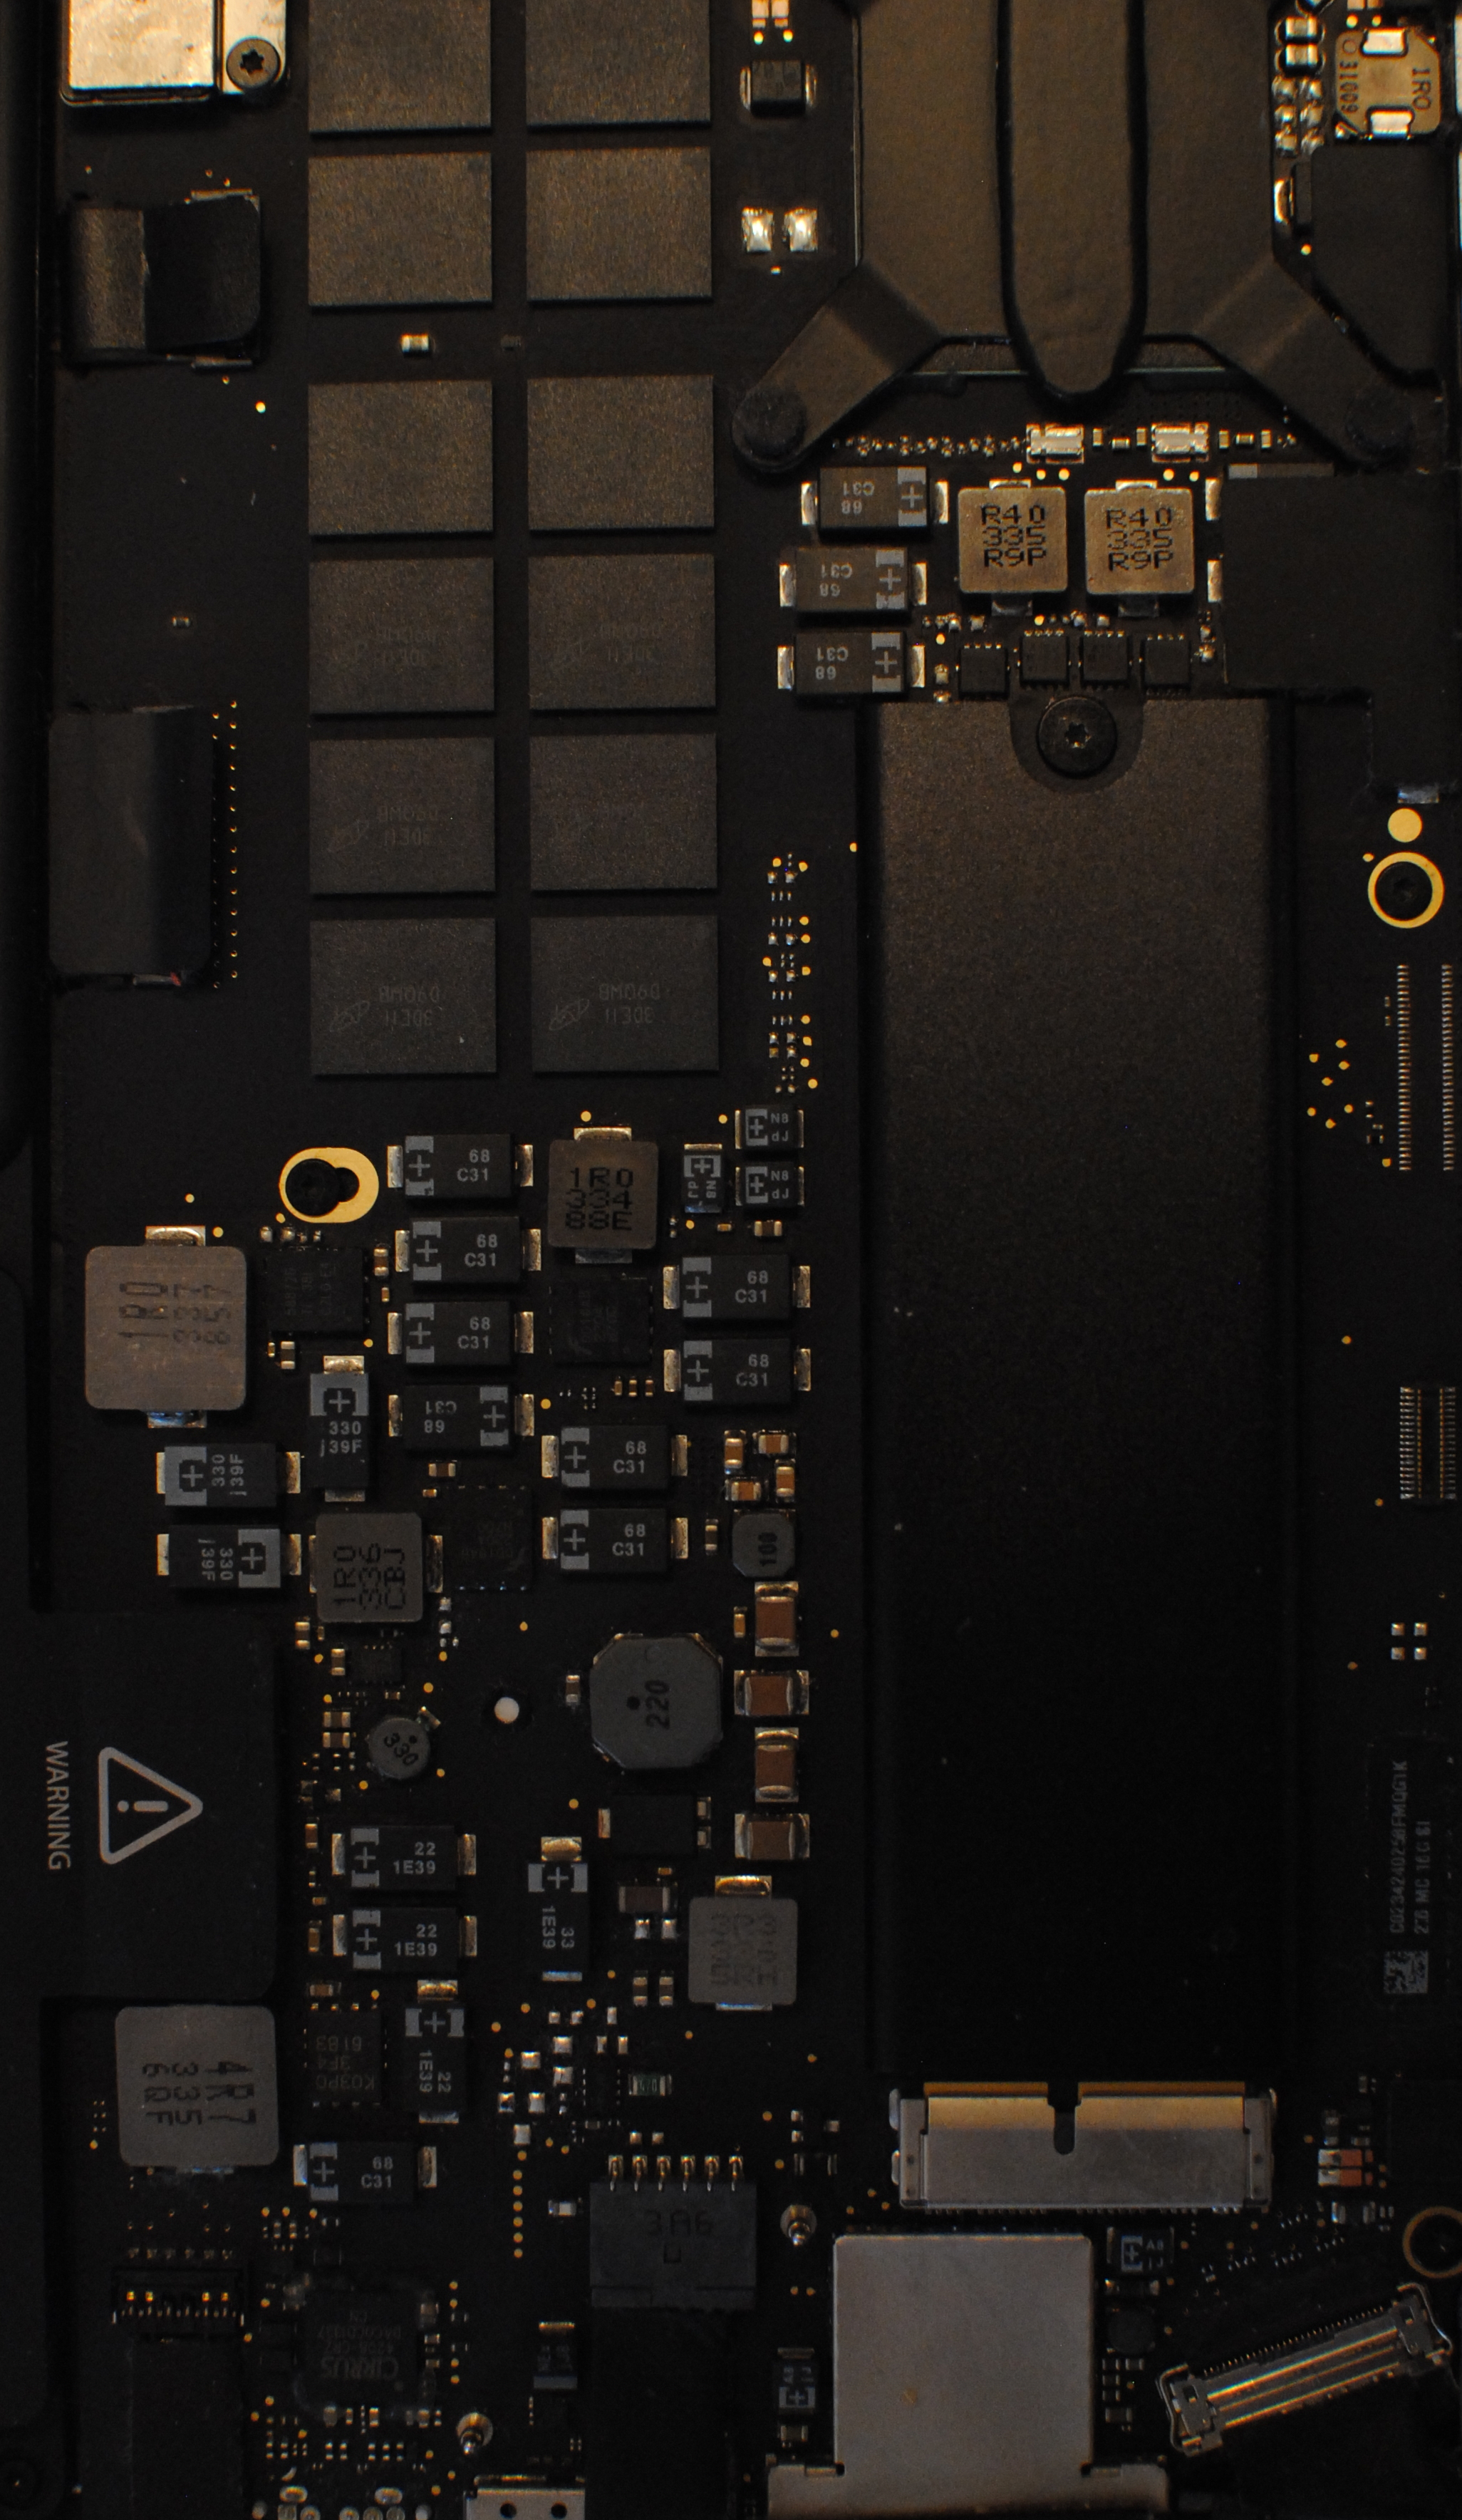
\includegraphics[scale=0.2]{figures/experiments/img.JPG}}
    
        \subfloat[Some cool related graphic]
        {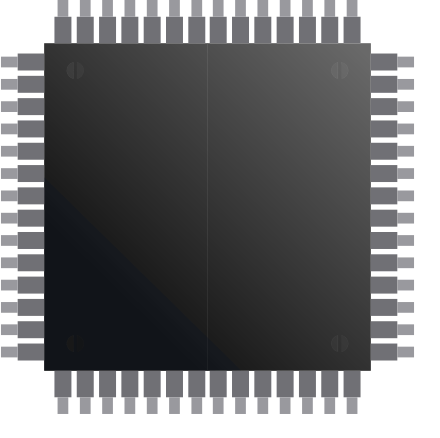
\includegraphics[scale=0.4]{figures/experiments/microcontroller.png}}
        \caption[Caption that appears in the figlist]{\textbf{Caption that appears under the fig} \lipsum[1-1]}
        \label{fig:pcaclasses}
    \end{centering}
\end{figure}

% \begin{table}[ht]
\centering
% spacing in table
\ra{1.3}
\begin{tabular}{@{}lr@{}}
  \toprule
  Type & Accuracy\\ \midrule
  A    & 82.47 $\pm$ 3.21 \\
  B    & 78.47 $\pm$ 2.43 \\
  C    & 84.30 $\pm$ 2.35 \\
  D    & 86.81 $\pm$ 3.01 \\
  \bottomrule
\end{tabular}

    \caption[Table caption]{\textbf{Table caption.} foo bar...\\}
    \label{tab:accuracy}
\end{table}

\section{VAE}

In the folling section I will present the results of my experiments with the Variational-Autoencoder to encode and decode actions from the environment.
Consistent over all experiments with the VAE sizes of the datasets are consistent:
\begin{itemize}
    \item train: 10.000 actions
    \item validation: 2000 actions
    \item test: 1000 action
\end{itemize}


\subsection{Pure Actions}

In every state of the sequential decision making process there are multiple actions available to go from the current state $s_t$ to the next state $s_{t+1}$ where the arm end position is at the goal position. To gain a dataset that contains such actions I sampled the robot arm angles in $s_t$ from a uniform distribution $\mathcal{U}_[0, 2\pi]$ and applied the CCD algorithm to get access to the action that leads from $s_t$ to $s_{t+1}$ with the robot arm end position near the goal state.\\

The results of the training process are shown in \figref{}

\subsection{Conditioning on States}

After watching the pure action encoding and decoding fail in the all important reconstruction loss. I got inspired by the paper \todo{cite LASER} and rerolled the experiments with an conditional Variational-Autoencoder where the conditional information is the information from $s_t$. 
The results of the training process are shown in \figref{}

We can observe that the test reconstruction loss is much lower that before and the kl loss

\begin{table}[]
    \centering
    \begin{tabular}{l|l|r|r}
         n & latent dim & r loss & kl loss\\
         2 & 2 & & \\
         2 & 1 & & \\
         5 & 5 & & \\
         5 & 4 & & \\
         5 & 3 & & \\
         5 & 2 & & \\
         5 & 1 & & \\
         10 & 2 & & \\
         10 & 2 & & \\
         10 & 2 & & \\
         10 & 2 & & \\
    \end{tabular}
    \caption{n is the number of joints, latent dimension is the size of the dimension the action is compressed to, r loss is the test reconstruction loss I used the MSE as the metric for the reconstruction loss, kl loss is the Kullback Leiber diveregence from the standard normal distribution on the test dataset}
    \label{tab:CVAE results}
\end{table}
\todo{Concering the table: make a lot of experiments so I can get an std ?, or should I just say that the training turns out to be not as stable as it should be in comparison to an VAE on MNIST and that we sampled runs until we got a good result?}

\subsection{Fitting Random Noise}

In this section I will present the results on how we tried to encode and decode actions sampled from a parameterized distributuion.
The idea is that in every state the agent can choose an action from $[-1, 1]^n$. Therefor I sampled a dataset independent and identically distributed from $\mathcal{U}^n_{[-1, 1]}$. this could be describe of trying to fit random noise.
The results for 800 epochs are shown in \figref{}.


\section{SAC}

\subsection{Hyperparameters}

\begin{table}[]
    \centering
    \begin{tabular}{l|l}
         name & values \\
         \hline
         task & ReachGoalTask, ImitationTask \\
         lr pi & 0.0005 \\
         lr q & 0.001 \\
         init alpha & 0.01 \\
         gamma & 0.98, 0  \\
         batch size & 32 \\
         buffer limit & 50000 \\
         start buffer size & 1000 \\
         train iteration & 20 \\
         tau & 0.01 \\ 
         target entropy & -40.0 \\
         lr alpha & 0.001 \\
         n epochs & 5000 \\
         action covariance mode & independent \\
         action covariance decay &  0.5 \\
         action magnitude & 0.1 \\
        \end{tabular}
    \caption{Hyperparameters for the Soft-Actor-Critic algorithm}
    \label{tab:Hyperparameters}
\end{table}
\todo{description?}

\subsection{Baseline}

In this section I want to present the results of the baseline experiments. To mimic a sequential decision making process and constrain the actions I manually tuned the parameter ``action magnitude'' between 1, 0.5, 0.2, and 0.1. The results are shown in figures: \figref{}

Stichworte die rein sollen
- Mit erhörter Anzahl an joint wid die Performance ober alle experimente immer schlechter
- Affällig hohe Varianz bei kleiner werdeneder Anzahl joint
- Absacken der Performance von 2 joints mit weiter Erniedrigung der action magnitude
- 5 joints scheinen eine ähnliche Performance über die action magnitude abzu geben
- Scheinbar habe ich bei 0.2 einen Wert gefunden der auch für höhere Anzahlen von joints gut zu funktionieren scheint. -> Fahre daher weiter mit diesem Parameter fort.

\begin{figure}
    \begin{center}
        \subfloat[Mean reward per step over the last 20 episodes.]{
            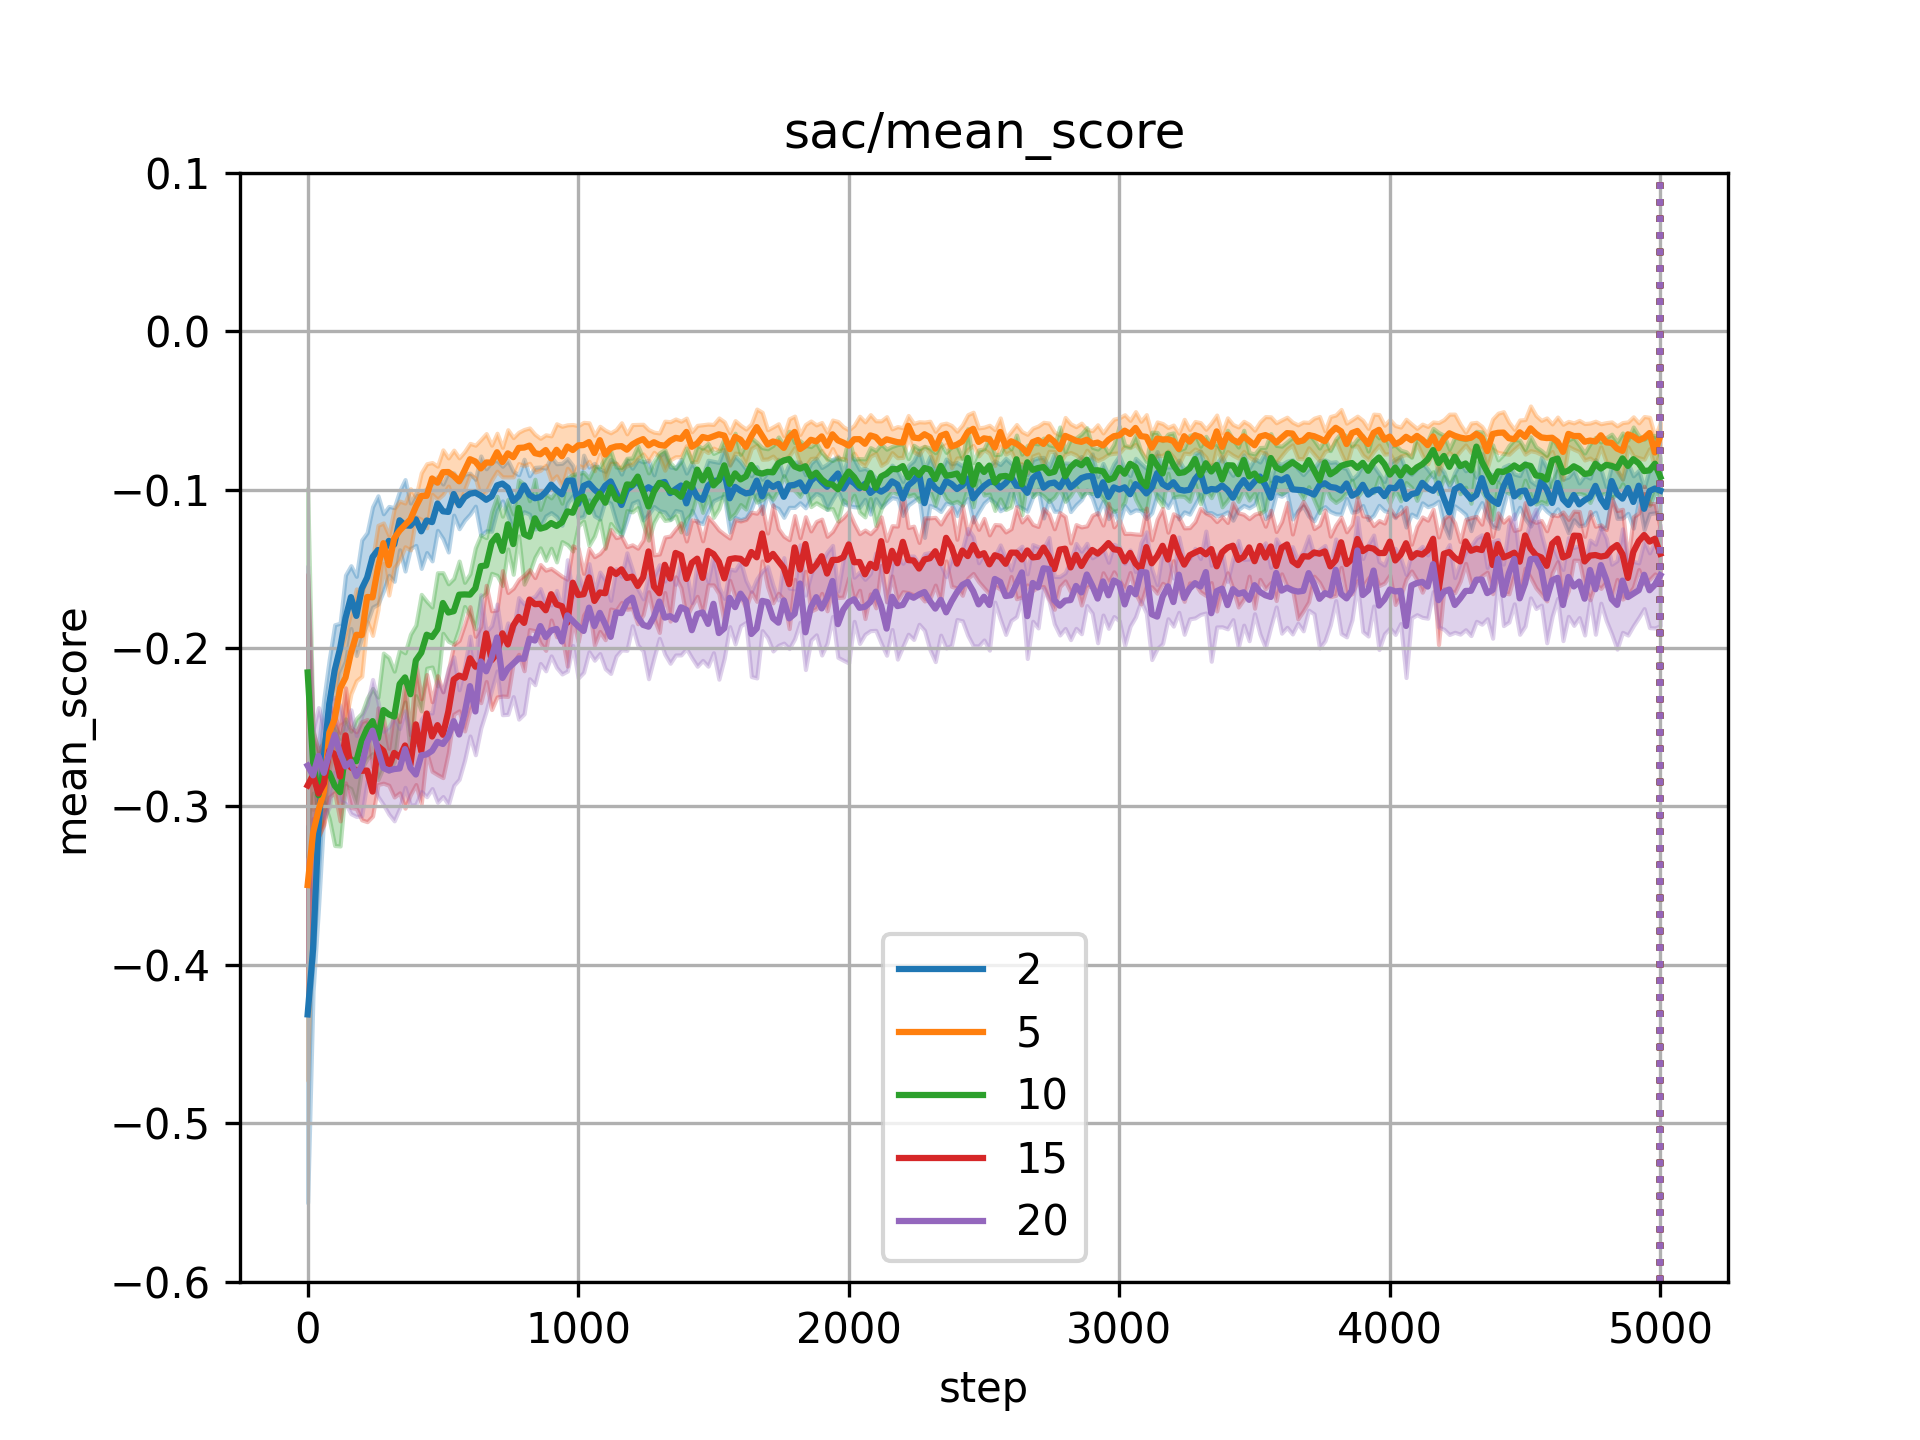
\includegraphics[width=0.46 \linewidth]{figures/experiments/sac_baseline_mean_score.png}
            \label{fig:SAC_baseline/reward}
            }
        \hfill
        \subfloat[Mean episode length over the last 20 episodes]{
        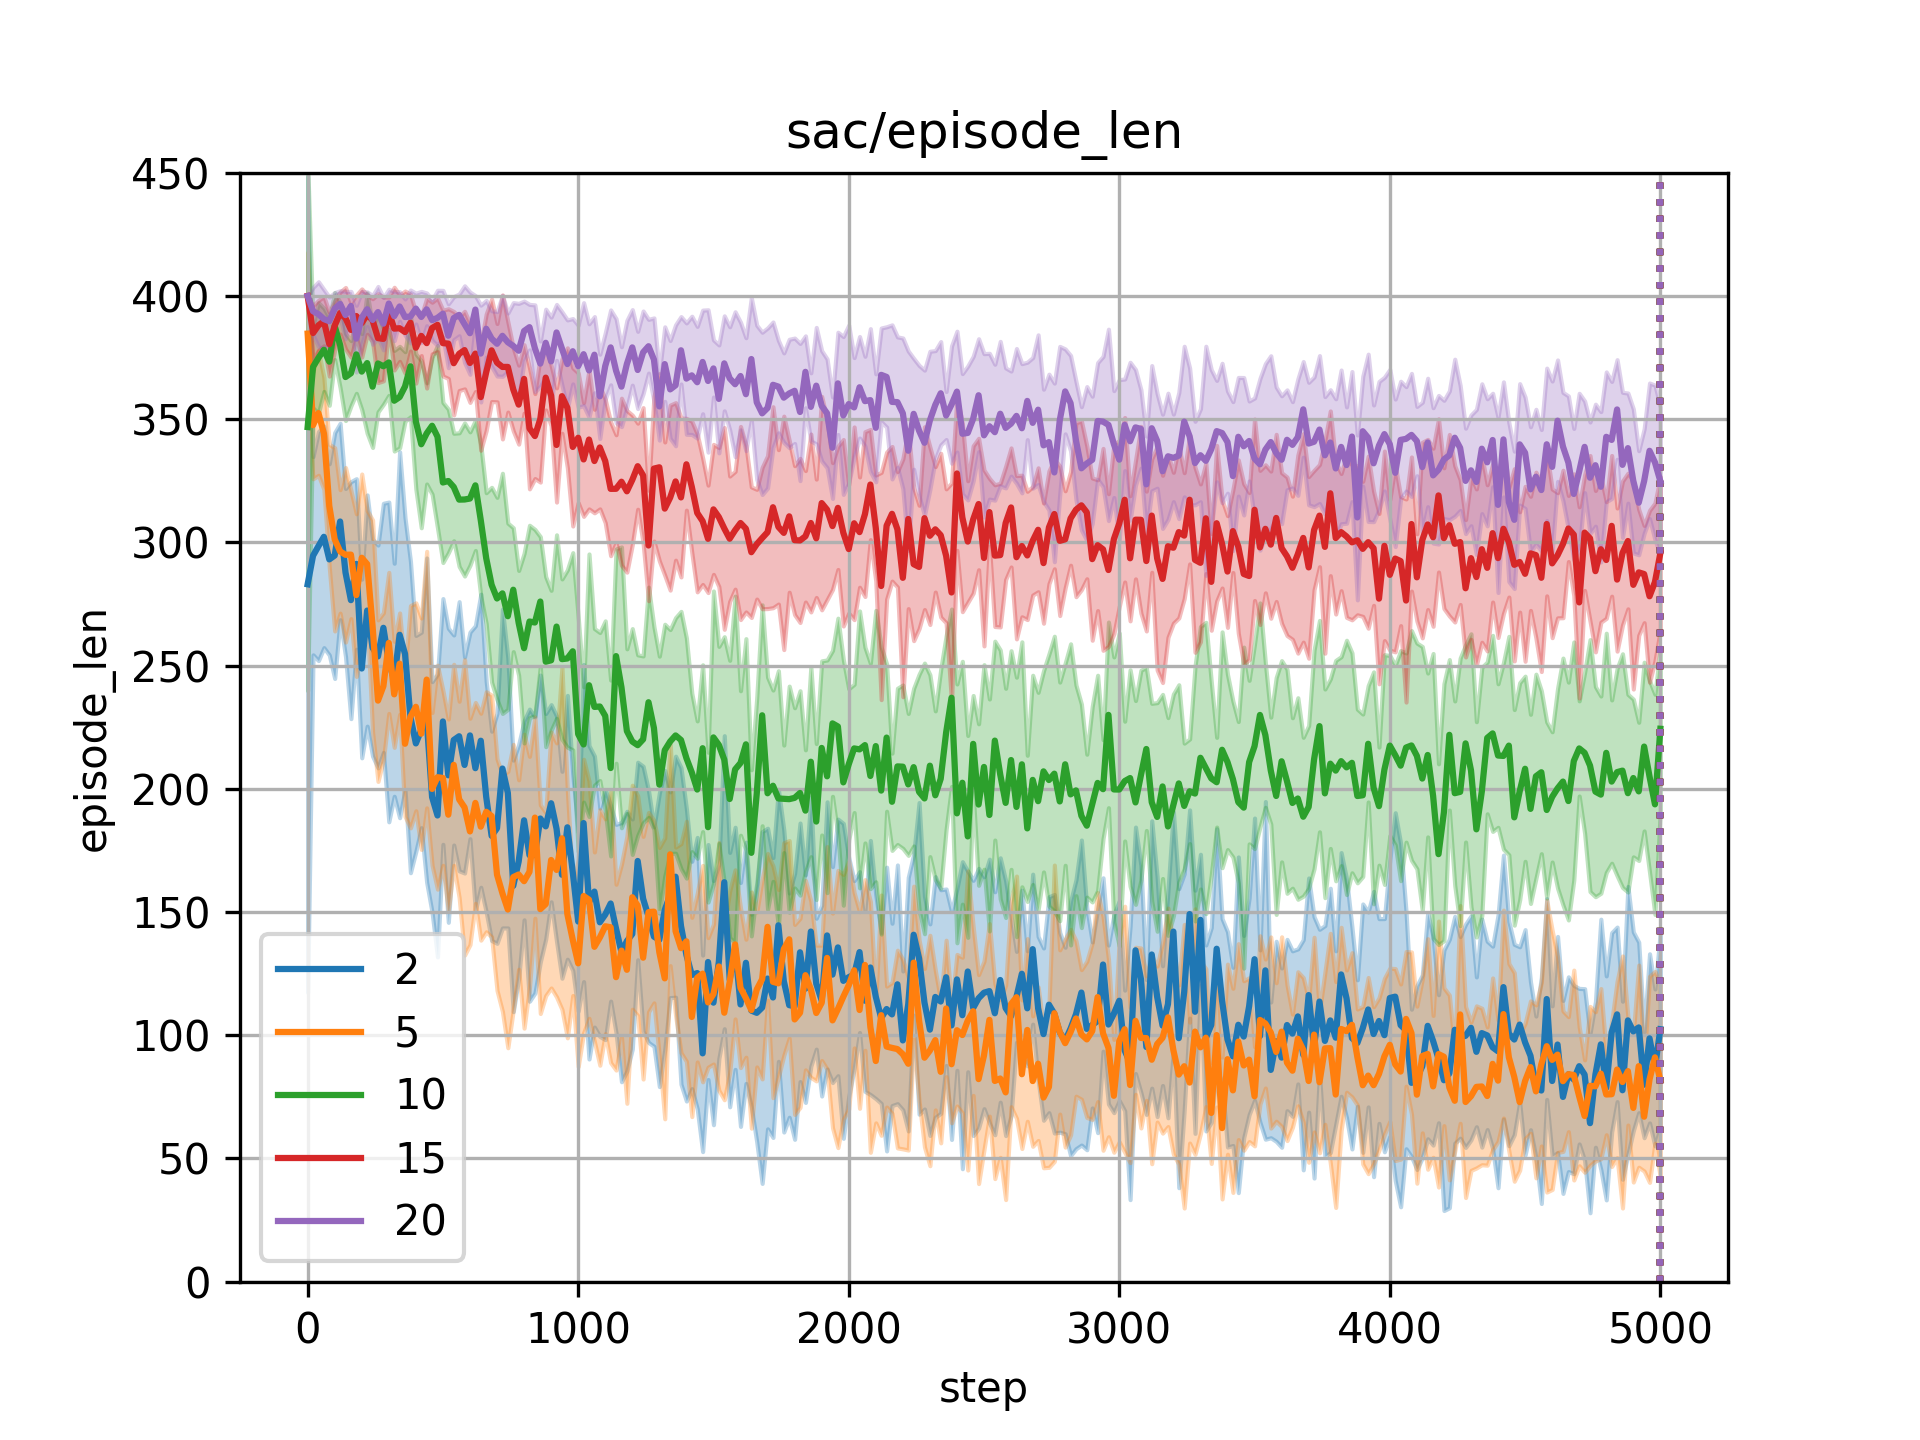
\includegraphics[width=0.46 \linewidth]{figures/experiments/sac_baseline_episode_len.png}
            \label{fig:SAC_baseline/episode_len}
            }
    \end{center}
    \caption[SAC baseline experiment results]{SAC baseline experiment results with an increasing number of joints. We can clearly see that the algorithm does not scale well with an increasing number of joints and therefor drops in performance. Each experiment was conducted 10 times and the shaded areas resemble the standard deviation around the mean.}
    \label{fig:SAC_baseline}
\end{figure}



